\documentclass[10pt,conference]{IEEEtran}
\usepackage[utf8]{inputenc}
\usepackage{graphicx,booktabs,amsmath,amssymb,url,xcolor}
\usepackage[hidelinks]{hyperref}
\graphicspath{{figures/}}

\newcommand{\todo}[1]{\textcolor{red}{\textbf{[TODO: #1]}}}
\newcommand{\unver}[1]{\textcolor{orange}{#1}}

\title{Silicon Core Harvesting is Visible in Supercomputer Telemetry:\\
A Fleet-Scale Study of 1{,}960 POWER9 Sockets}

\author{\IEEEauthorblockN{Mohsen Seyedkazemi Ardebili}
\IEEEauthorblockA{\textit{Affiliation} \\ \texttt{mohsen.seyedkazemi@gmail.com}}
\and
\IEEEauthorblockN{\todo{co-authors}}
\IEEEauthorblockA{}}

\begin{document}
\maketitle

\begin{abstract}
Processor vendors sell partially defective dies by permanently disabling faulty units, a practice
known as core harvesting. The resulting per-die disable maps are proprietary and are conventionally
invisible to system owners. We show that the out-of-band (BMC/IPMI) sensor telemetry routinely
collected by production supercomputers exposes these maps directly, and we recover them for all
1{,}960 processor sockets of CINECA's Marconi100 from the public M100 ExaData
release~\cite{borghesi2023m100}. Every socket exposes exactly 16 of 24 possible per-core thermal
sensors, and the eight absent sensors always form four complete \emph{slice} pairs
$(2k,2k{+}1)$---the POWER9 unit that shares an L2/L3 block~\cite{thompto2016power9,wikichip_power9}---with
zero exceptions. We observe 442 of the 495 combinatorially possible patterns, establishing that the
map is per-die rather than a fixed SKU. Using a curveball null that preserves both per-socket and
per-slice marginals, we show harvested slices cluster in sensor-index space ($z=-20.8$). Thermal
analysis confirms that the two cores of a slice are physically abutted (residual correlation
$r=+0.51$ within-slice versus $+0.29$ for cross-slice neighbours at identical index distance), but
we find only weak evidence that the slice index itself is monotonic in physical die position
($p=0.025$; a $3\times4$ grid fits the thermal coupling better than a linear arrangement).
We detect a sharp procurement-lot boundary at rack~22 (Welch $t=27.3$) separating two populations
with markedly different harvesting statistics. Finally, tracking every socket across the full
2.5-year, 1.67-million-socket-day record, we find harvest maps behave as near-static manufacturing
constants: 89.5\% of sockets never change configuration, and \textbf{none of the 235 observed
transitions occurs during operation}---every one coincides with a reboot. Against that backdrop we
isolate \textbf{three episodes, on three of 1{,}968 sockets, in which a socket ran on 14 cores for
2--4 days}, each losing exactly one slice and at least one subsequently restored: to our knowledge
the first direct observation of POWER9 field core-guarding in a production system, at a measured
rate of 0.15\% of sockets over 2.5 years.
\end{abstract}

\begin{IEEEkeywords}
core harvesting, silicon binning, HPC telemetry, POWER9, yield, hardware provenance
\end{IEEEkeywords}

\section{Introduction}
Every large processor die ships with defects. Rather than discard them, vendors permanently fuse
off the faulty units and sell the remainder as a lower-core-count part---\emph{core harvesting}.
The practice is universal and openly acknowledged, but the resulting \emph{per-die} maps of which
units were disabled are proprietary: a buyer is told the part has 16 cores, never \emph{which} 16.
Those maps encode information about a fab's defect process, a vendor's binning policy and a
procurement's provenance that is otherwise unavailable outside the manufacturer.

Independently, HPC operators have begun publishing holistic out-of-band monitoring at fleet
scale~\cite{borghesi2023m100}. We observe that such telemetry carries an unintended side channel:
a baseboard management controller exposes one thermal sensor per \emph{physical} core position and
does not renumber the surviving cores compactly, so the set of sensors that report \emph{is} the
die's harvest map, published inadvertently and at fleet scale.

We exploit this to recover harvest maps for every processor socket of CINECA's Marconi100, a
Top-10 system, from a public dataset, and to track them across 858 days. Our contributions are:

\begin{itemize}
\item A recovery method (Sec.~\ref{sec:method}) with an explicit validity argument, needing only
      per-core sensor telemetry that operators already collect.
\item The first fleet-scale characterisation of core harvesting in a deployed supercomputer: the
      granularity is exactly the POWER9 slice, maps are per-die rather than per-SKU, and harvested
      slices cluster in sensor-index space.
\item Evidence of \emph{procurement-lot structure}---a sharp changepoint separating two
      populations with markedly different binning statistics---from telemetry alone.
\item A longitudinal result over 1.67\,M socket-days: maps are static, configuration changes occur
      only at reboot, and three field core-guard episodes are isolated and corroborated.
\item A negative result that matters operationally: the harvest map has no practical effect on
      socket power (Sec.~\ref{sec:impact}), so schedulers need not model it.
\end{itemize}

\section{Background}
\subsection{POWER9 slice organisation}
The POWER9 die used in the IBM Power System AC922 contains 24 SMT4 cores (equivalently 12 SMT8
cores) on a $695\,\mathrm{mm}^2$ die in 14\,nm FinFET with 17 metal layers~\cite{wikichip_power9}.
Critically, \emph{each pair of SMT4 cores---or one singleton SMT8 core---comprises a}
slice\emph{, and each slice owns 512\,kB of L2 and 10\,MB of
L3}~\cite{wikichip_power9,thompto2016power9}. IBM's Hot Chips 28 presentation shows the 24 cores
above 12 $\times$ 10\,MB L3 blocks, attached to a 7\,TB/s on-chip fabric at
$256\,\mathrm{GB/s}\times12$~\cite{thompto2016power9}. The slice is therefore the natural fusing
granularity: disabling one SMT4 core would strand its half of a shared L2/L3 block.

Marconi100 nodes are AC922 model 8335-GTG with $2\times$ 16-core POWER9 at 2.6/3.1\,GHz and
$4\times$ NVIDIA V100~\cite{ibm_ac922,cineca_m100}. \textbf{A 16-core part is a 24-core die with
four slices fused off}; this is the object of our study. Fig.~\ref{fig:schematic} shows the
organisation annotated with the harvest rates we measure.

\subsection{The M100 ExaData dataset}
M100 ExaData~\cite{borghesi2023m100} publishes 49.9\,TB of telemetry from Marconi100 covering
2020-03 to 2022-09 across 980+ nodes. The IPMI plugin collects BMC sensor data at 20\,s cadence.
The documentation describes the core-temperature family as \texttt{pX\_coreY\_temp}, ``Temperature
of core n.\ Y in the CPU socket n.\ X. X=0..1, Y=0..23''~\cite{exadata_repo}. \emph{This specifies
the BMC sensor-ID namespace, not the active core count}---the distinction is the entry point for
this study.

\section{Method}
\label{sec:method}
\subsection{Recovering the disable map}
For each month we enumerate the \texttt{metric=pX\_coreY\_temp} partitions and count samples per
(node, socket, core). A core index is \emph{present} for a socket if it emits any sample in the
window. We define the disable map of socket $s$ as $M[s,k]\in\{0,1\}^{12}$ over slices
$k=\lfloor \mathrm{core}/2 \rfloor$.

The key validity argument is that \textbf{the BMC does not renumber active cores compactly}: were
that so, every socket would report indices 0--15. Instead we observe arbitrary 16-element subsets
of $\{0,\dots,23\}$, so the index is a fixed physical-position identifier.

\subsection{Null model for clustering}
Every socket has exactly four harvested slices, so the constraint induces negative dependence and a
naive independence null is invalid. We use the curveball algorithm~\cite{strona2014curveball},
which preserves \emph{both} row sums (4 per socket) and column sums (per-slice marginals) while
randomising association structure. Row- and column-sum preservation is asserted on each of 200 draws.

\subsection{Thermal probing of die topology}
Cores on a socket share workload and inlet air, producing a dominant common mode. We remove it by
subtracting the per-timestamp cross-core mean, double-centre, and compute residual correlations.
Physically abutted cores should retain positive residual coupling.

\paragraph*{Caveat} Common-mode removal forces each row of the residual matrix to sum to
approximately zero, so negative values at large index gaps are partly mechanical. We therefore rely
on contrasts \emph{at identical index distance}, which control for this exactly.

\section{Results}

\begin{figure*}[t]\centering
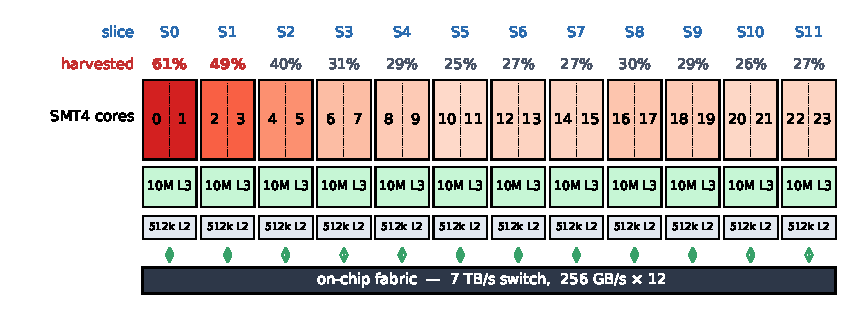
\includegraphics[width=\textwidth]{f1_slice_schematic.pdf}
\caption{POWER9 slice organisation (after~\cite{thompto2016power9}) annotated with the measured
per-slice harvest rate across 1{,}960 Marconi100 sockets. Each slice holds two SMT4 cores sharing
512\,kB L2 and 10\,MB L3 on a common fabric port. Harvesting always removes whole slices.
\textbf{The horizontal ordering is the IPMI sensor index, which we show is \emph{not} established
as the physical die ordering} (Sec.~\ref{sec:layout}).}
\label{fig:schematic}
\end{figure*}

\subsection{Every socket is 16 cores; granularity is the slice}
\paragraph*{Populations} Three socket populations recur and are kept distinct throughout:
$\mathcal{S}_{\text{all}}$, the 1{,}968 sockets appearing anywhere in the record (984 nodes);
$\mathcal{S}_{\text{map}}$, the 1{,}962 with at least one clean day and hence a well-defined
harvest map; and $\mathcal{S}_{2004}$, the 1{,}960 present in the single month 2020-04. All
structural results below are over $\mathcal{S}_{\text{map}}$ and the full 31-month record.

\begin{table}[h]\centering\caption{Disable-map structure over the full 31-month record.}
\begin{tabular}{lr}\toprule
Sockets with a well-defined harvest map & 1{,}962\\
Median clean days supporting each map & 775\\
Socket-days reporting exactly 16 cores & \textbf{99.985\%}\\
Sockets ever reporting 24 cores & 0\\
Harvested cores form complete $(2k,2k{+}1)$ pairs & \textbf{1{,}962 (100\%)}\\
\bottomrule\end{tabular}\end{table}

The perfect pair structure is the central mechanical finding: it matches the POWER9 slice
definition exactly and rules out per-core fusing.

\subsection{The map is per-die, not per-SKU}
\textbf{443} distinct patterns appear among the $\binom{12}{4}=495$ possible
(Fig.~\ref{fig:rank}). The most common (slices 0--3) covers only 5.5\% of sockets. Within a node the two sockets match in just
1.2\% of cases, with mean overlap 1.648 slices against a shuffled null of $1.474\pm0.026$
($z=+6.6$)---nearly independent, with a small excess attributable to same-lot pairing.

\subsection{Marginals are strongly non-uniform}
Slice~0 is harvested on 61.2\% of sockets against a uniform expectation of 33.3\%
($\chi^2=807.2$, $\mathrm{df}=11$, $p\ll0.001$); Fig.~\ref{fig:marg} splits this by lot. These
marginals are remarkably stable in time: across the 31 months the largest standard deviation of any
slice's monthly rate is \textbf{0.25 percentage points}, and slice~0 ranges only 60.9--61.8\%
(Fig.~\ref{fig:stab}). The single-month snapshot used in earlier drafts was therefore
representative, and every estimate here is a 2.5-year-stable measurement.

\subsection{Harvested slices cluster in index space}
\label{sec:cluster}
Under the curveball null the mean index gap between harvested slices is $4.242$ versus
$4.582\pm0.017$ ($z=-20.2$). Applying a Bonferroni correction across all $\binom{12}{2}=66$ pair
tests ($|z|>3.83$), 17 pairs remain significant (Fig.~\ref{fig:cooc}). The positive excesses are
0\&1 ($z=+16.7$), 6\&7 ($+9.2$), 2\&3 ($+8.0$), 8\&9 ($+7.7$), 10\&11 ($+7.5$), 4\&5 ($+7.1$),
1\&2 ($+6.9$) and 0\&2 ($+6.3$): \textbf{eight of the nine positive-excess pairs have
$|\Delta k|\le2$}, and every significant \emph{deficit} is a distant pair. We report the single
exception rather than rounding it away.

\subsection{Slice siblings are physically abutted}
Fig.~\ref{fig:thermal} shows residual correlation against core index distance. At \emph{identical}
distance of~1, within-slice siblings reach $r=+0.51$ versus $+0.29$ for cross-slice neighbours;
per-node the contrast between near ($\le2$) and far ($\ge12$) pairs is $+0.45\pm0.20$ with
40/40 nodes positive (paired $t=+13.9$). The two cores of a slice are roughly twice as coupled as
equally-numbered cores across a slice boundary, confirming both physical abutment and the slice as
a physical unit.

\subsection{The slice index is \emph{not} established as the physical ordering}
\label{sec:layout}
Free classical MDS on the pooled $24\times24$ matrix is dominated by noise (leading axis 20.5\% of
variance, correlation with core index only $+0.34$), so we instead score explicit candidate
floorplans by correlating predicted physical distance against measured thermal coupling
(Fig.~\ref{fig:layout}). The identity $1\times12$ linear arrangement scores $-0.271$, better than a
random ordering ($z=-2.22$, $p=0.025$) but \emph{worse} than a $3\times4$ grid ($-0.565$); a
hill-climbing search finds an ordering scoring $-0.715$ whose rank correlation with the identity
ordering is only $+0.34$.

\textbf{We therefore do not claim the sensor index is monotonic in physical die position.} The
index-space clustering of Fig.~\ref{fig:cooc} is a robust empirical fact, but its interpretation as
\emph{spatial} defect clustering is not established by our data and must be stated as a hypothesis.
\todo{obtain an annotated POWER9 die shot or OpenBMC sensor-ID mapping to settle this.}

\subsection{A procurement-lot boundary at node 440}
\label{sec:lot}
Node IDs map to position as $\mathrm{rack}=\lfloor \mathrm{id}/20\rfloor$~\cite{exadata_repo}. A
changepoint scan maximises Welch $t$ at rack~22 (node~440), $t=26.6$ (Fig.~\ref{fig:rack}).

\begin{table}[h]\centering\caption{Two populations either side of the lot boundary.}
\begin{tabular}{lrrr}\toprule
Population & Sockets & $P(\text{slice 0})$ & Distinct patterns\\\midrule
Lot A (racks 0--21) & 880 & 88.2\% & 230\\
Lot B (racks 22--48) & 1{,}082 & 39.3\% & 416\\
\bottomrule\end{tabular}\end{table}

Lot A marginals fall steeply with slice index; Lot B is nearly flat. Permutation tests confirm
between-rack heterogeneity for slices 0, 1, 2, 5 ($p<0.01$), and same-rack sockets share more
harvested slices than chance ($1.568$ vs $1.454\pm0.008$, $z=+14.1$).

\subsection{Configuration lifetime}
\label{sec:lifecycle}
POWER9 exposes mechanisms that \emph{could} alter the active set after manufacture: predictive
Dynamic Processor Deallocation, persistent GARD records read by hostboot at IPL and clearable with
\texttt{opal-gard}, and the field core override used for licensing~\cite{ibm_deconfig,skiboot_gard}.
Operating-system core offlining is invisible to the BMC and cannot affect sensor presence. Whether
harvest maps are static in practice is therefore an empirical question, which we answer by
aggregating every core sample to (node, socket, day) counts across the dataset.
All numbers in this section are over the complete 31-month record (2020-03 to 2022-09).

\paragraph{The count is very nearly invariant} Across all 31 months---1{,}671{,}297 socket-days
over 858 days and 984 nodes---\textbf{99.985\% report exactly 16 active cores}. Of the 256
exceptions, 39 have an odd count, which \emph{cannot} arise from slice-granular fusing and
therefore proves the collector can drop individual cores; the counts above 16 are unions spanning a
same-day reconfiguration. Only \textbf{nine} socket-days are fully-sampled with an even count below
16, and these are the subject of the guard analysis below.

\paragraph{Configurations are near-static} Restricting to \emph{clean} socket-days (16 cores, each
at $>$90\% of the 4{,}320 samples expected at 20\,s cadence) leaves 1{,}517{,}473 socket-days, a
median of 775 observed days per socket. \textbf{89.5\% of sockets never change configuration}
(1{,}756 of 1{,}962); 183 have two distinct sets, 19 have three, three have four and one has five.

\paragraph{Three core-guard episodes} The nine anomalous socket-days resolve into
\textbf{three sustained episodes on three distinct sockets}, each with the exact signature of a
field deconfiguration (Table~\ref{tab:guard}). In every case the socket loses \emph{exactly one
slice}---a complete $(2k,2k{+}1)$ pair---runs on 14 cores for 2--4 consecutive fully-sampled days,
and in at least one case the slice is subsequently restored, consistent with an operator clearing
the GARD record~\cite{skiboot_gard}. The measured rate is \textbf{3 episodes across 1{,}968
sockets over 2.5 years}, i.e.\ 0.15\% of sockets. Durations are lower bounds, since an episode is
counted only on fully-sampled days.

\emph{Ruling out a collector fault.} The competing explanation is that the collector dropped
exactly those two metric streams. We test it directly: for each episode we ask whether the
\emph{other} sensors on the same node---in particular on the same socket---kept reporting. They
did. In all three episodes the two slice sensors read zero for the entire window while
\textbf{all ten control metrics, including \texttt{pX\_power} and \texttt{pX\_vdd\_temp} on the
same socket, sustained a full 4{,}320 samples per day} (Fig.~\ref{fig:guard}). A collection fault
that silences precisely the two cores of one slice for several consecutive days, while leaving
every other sensor on the same socket at full cadence, is not a plausible account. We therefore
attribute these episodes to hardware deconfiguration; to our knowledge this is the first direct
observation of POWER9 field core guarding in a deployed system.

\begin{table}[h]\centering\caption{Core-guard episodes. Baselines are the adjacent observed day,
not the socket's global modal set, since two of these sockets also change configuration elsewhere
in their life.}\label{tab:guard}
\begin{tabular}{llrlr}\toprule
Socket & Dates & Days & Slice lost & Restored\\\midrule
347\,p1 & 2020-03-13--16 & 4 & 4 (cores 8,9)   & yes\\
411\,p1 & 2021-11-13--15 & 3 & 6 (cores 12,13) & yes$^\dagger$\\
946\,p0 & 2020-08-31--09-01 & 2 & 8 (cores 16,17) & not observed\\
\bottomrule\end{tabular}
\\[2pt]\footnotesize$^\dagger$restored via a day that also spans a reconfiguration.
\end{table}

\paragraph{Changes never occur during operation} Of \textbf{235} transitions across the full
record, \textbf{zero} occur between consecutive reporting days: every one coincides with a gap in
reporting (median 2\,d), against a background in which only 4.2\% of consecutive reporting days
are more than one day apart. Configuration changes
are boot-time events, exactly as the guard/deconfiguration mechanism predicts.

The only two apparent counterexamples confirm the rule once examined at full timestamp resolution.
Nodes~315 (p1) and~342 (p0) appear to change within a single day, and produce the dataset's only
20- and 22-core socket-days. In fact both cut over on 2021-03-02 across a \emph{sub-day reporting
gap}: on node~315 the outgoing cores $\{4,5,20,21\}$ report until 08:42 and the incoming cores
$\{8,9,10,11\}$ resume at 09:10, a 28-minute outage, with exactly 16 cores before and 16 after; the
20/22-core counts are unions across the cutover. Node~342 cuts over in the same window, indicating
a coordinated maintenance reboot. Day-granularity aggregation is therefore \emph{conservative}
here: it cannot see sub-day downtime, so our transition-gap statistics understate how consistently
changes coincide with reboots.

\paragraph{Changes concentrate on a few dates} The 235 transitions involve 132 nodes on 81
distinct dates, but are heavily clustered: 2020-03-20 alone accounts for 63 and the top three dates
for 41\%. Such synchronised, fleet-wide changes are more consistent with an administrative or
firmware event than with independent per-node hardware work (see OI-2).

\paragraph{Some apparent changes are socket relabelling} When node~$n$'s socket p0 loses exactly
the slices p1 gains and vice versa, the dies are unchanged and only the p0/p1 labels have swapped.
This accounts for \textbf{20\%} of the 230 transitions where both sockets are observable.

\paragraph{Caveat} An apparent change can arise from (a)~genuine hardware reconfiguration,
(b)~socket relabelling, or (c)~a change in the BMC sensor-ID mapping, e.g.\ after a firmware
update. The tight clustering of 86 transitions into three days is consistent with (c) and we
cannot separate these from telemetry alone. \todo{seek CINECA maintenance logs for March 2020.}

\begin{figure}[t]\centering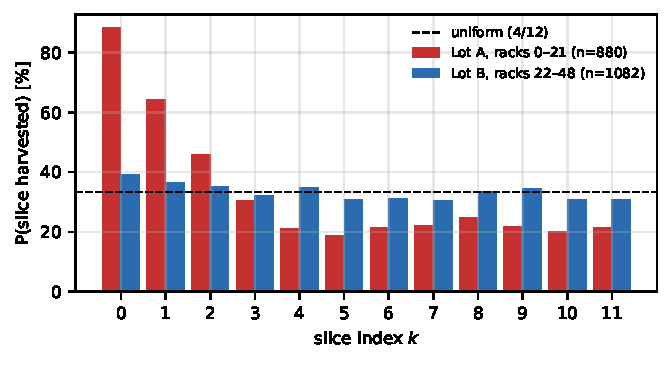
\includegraphics[width=\columnwidth]{f2_marginals.pdf}
\caption{Per-slice harvest probability by procurement lot.}\label{fig:marg}\end{figure}

\begin{figure}[t]\centering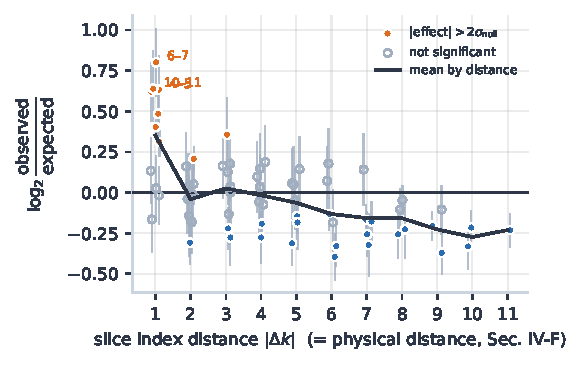
\includegraphics[width=.85\columnwidth]{f3_cooccurrence.pdf}
\caption{Co-harvest $z$ against the curveball null. Excess is confined to near-diagonal
(index-adjacent) slice pairs.}\label{fig:cooc}\end{figure}

\begin{figure}[t]\centering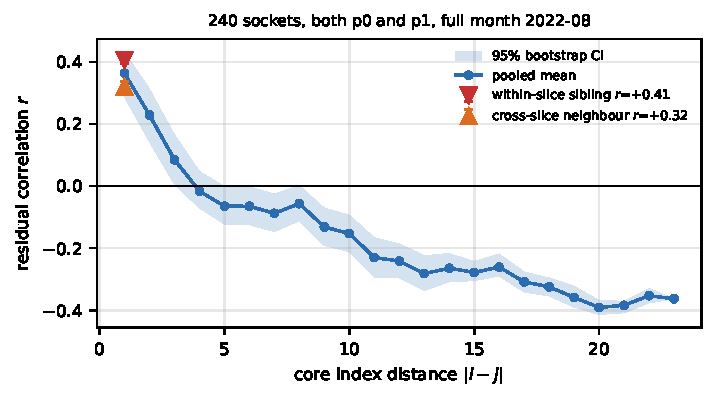
\includegraphics[width=\columnwidth]{f4_thermal_decay.pdf}
\caption{Residual thermal correlation versus core index distance. The within- versus cross-slice
contrast at distance~1 controls exactly for index gap.}\label{fig:thermal}\end{figure}

\begin{figure}[t]\centering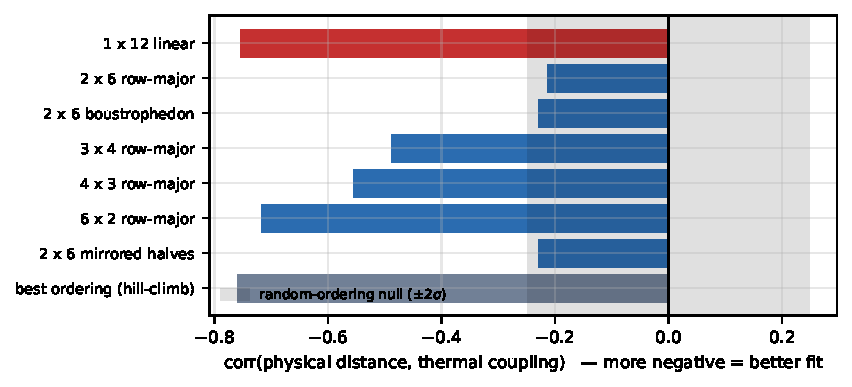
\includegraphics[width=\columnwidth]{f5_layout_hypotheses.pdf}
\caption{Candidate floorplans scored against measured thermal coupling. The linear index ordering
(red) beats a random ordering only marginally and is outperformed by a $3\times4$ grid.}
\label{fig:layout}\end{figure}

\begin{figure}[t]\centering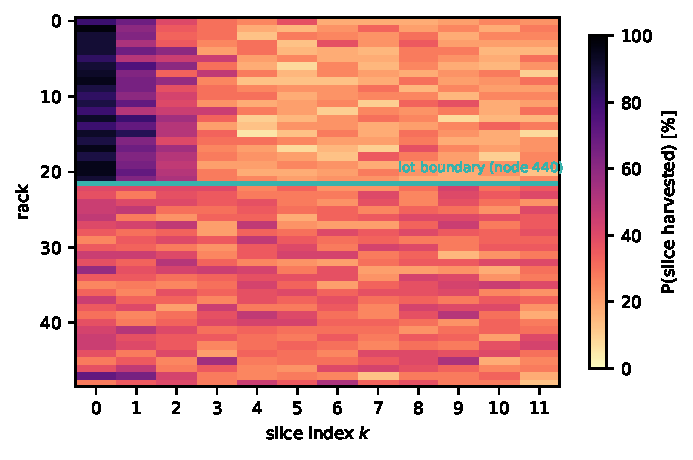
\includegraphics[width=\columnwidth]{f6_rack_heatmap.pdf}
\caption{Harvest probability by rack and slice. The lot boundary at rack~22 is
visible as an abrupt change.}\label{fig:rack}\end{figure}

\begin{figure}[t]\centering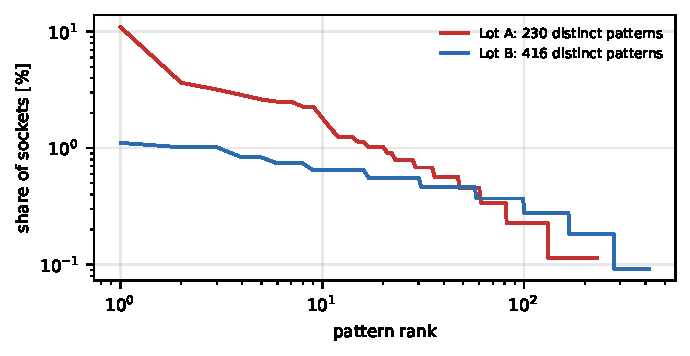
\includegraphics[width=\columnwidth]{f7_pattern_rank.pdf}
\caption{Rank--frequency of disable patterns. Lot B is markedly more diverse.}\label{fig:rank}\end{figure}

\subsection{The harvest map has no operational consequence}
\label{sec:impact}
Recovering a hidden hardware property is only useful if it changes something. We therefore ask
whether the harvest map predicts socket behaviour, using a \textbf{within-node paired contrast}:
the two sockets of a node share chassis, airflow, inlet air, power supply and---to first
order---workload, so the difference $p_0-p_1$ removes the node-level confounds that make
cross-node power comparisons unreliable. We summarise each socket's map by the mean index of its
active slices, their dispersion, the number of adjacent active pairs, and the count of active
slices in the low half, and correlate the socket-to-socket difference in each against the
socket-to-socket difference in mean CPU power over six months (5{,}880 node-months,
Fig.~\ref{fig:impact}).

The associations are statistically detectable and practically negligible. The strongest is between
the mean active-slice index and socket power: $r=+0.039$ (permutation $p=0.003$), explaining
\textbf{0.16\% of variance}, with a slope of $+0.46$\,W per unit of slice index
(95\% CI $[+0.16,+0.76]$). Across the full observed range of the predictor this is
\textbf{3.1\,W}, against a socket-to-socket power spread of 17.8\,W. For calibration, the same
paired design shows socket~p0 draws $7.7$\,W more than socket~p1 on average ($t=44.6$)---mere
physical position in the chassis matters more than twice as much as the entire range of harvest-map
variation.

We therefore report a deliberate negative result: \textbf{harvest maps are operationally
invisible}. Schedulers, power models and node-ranking heuristics need not represent them, and
node-to-node performance variability in this system must be sought elsewhere. The result also
strengthens the provenance interpretation of Sec.~\ref{sec:lot}: because the map has no
behavioural footprint, the lot boundary cannot be an artefact of operational differences between
racks.

\section{Discussion}
\paragraph{Why is slice 0 special?} The single most striking number is that slice~0 is harvested on
88.2\% of Lot~A sockets but only 39.3\% of Lot~B. Two explanations are live. Under
\emph{defect-driven} harvesting, fusing follows wherever killer defects land; this is supported by
the index-adjacency clustering of Sec.~\ref{sec:cluster} and by Lot~B's nearly flat marginals,
which are close to what a spatially random defect process would give. Under \emph{policy-driven}
harvesting, slice~0 abuts a shared structure and is preferentially fused for reasons of yield
policy, binning recipe, or physical design; an 88\% rate on one specific slice is very hard to
obtain from random defects. The data are consistent with Lot~A being policy- or
recipe-dominated and Lot~B defect-dominated, i.e.\ with a change of binning recipe or die source
between the two procurements. We cannot settle this from one machine and report both.

\paragraph{The direction of causation is fixed.} A tempting objection to Sec.~\ref{sec:lot} is that
rack position is confounded with cooling and workload. It cannot be: harvesting is performed by
fusing at manufacture, months before a part is installed, so nothing about a socket's position in
the machine room can influence its harvest map. The only admissible causal direction runs from
procurement batch to rack, which is precisely the provenance signal we claim.

\paragraph{What this buys an operator.} Three things. Fleet telemetry can audit a procurement
without vendor cooperation, detecting whether a delivery is homogeneous. It can detect field
deconfiguration events that would otherwise be visible only in service logs. And, per
Sec.~\ref{sec:impact}, it establishes when a hardware property can safely be \emph{ignored}.

\section{Related work}
\todo{expand; the citations below are located but \unver{unverified}.}
Manufacturing variability in HPC has been studied mainly through its
\emph{performance} consequences---frequency and power spread under a power
cap~\unver{\cite{inadomi2015variation}}, turbo-boost variation across nominally identical
processors~\unver{\cite{acun2016variation}}, and accelerator-level variability in GPU-rich
systems~\unver{\cite{sinha2022gpuvariability}}. That literature treats the die as a black box
characterised by its behaviour. Yield modelling, conversely, treats defect statistics directly:
the negative-binomial family~\unver{\cite{stapper1993negbinom}} and spatial wafer-map
models~\unver{\cite{friedman2007waferyield}} describe clustered killer defects but are validated on
fab data unavailable to system owners. To our knowledge no prior work recovers per-die harvesting
maps from deployed-system telemetry, which is the gap this paper addresses.

\begin{figure}[t]\centering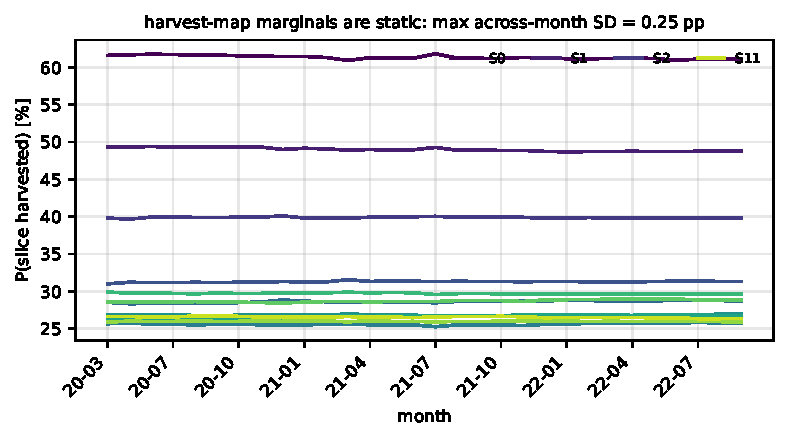
\includegraphics[width=\columnwidth]{f8_month_stability.pdf}
\caption{Per-slice harvest rate in each of the 31 months. The largest across-month standard
deviation of any slice is 0.25 percentage points.}\label{fig:stab}\end{figure}

\begin{figure}[t]\centering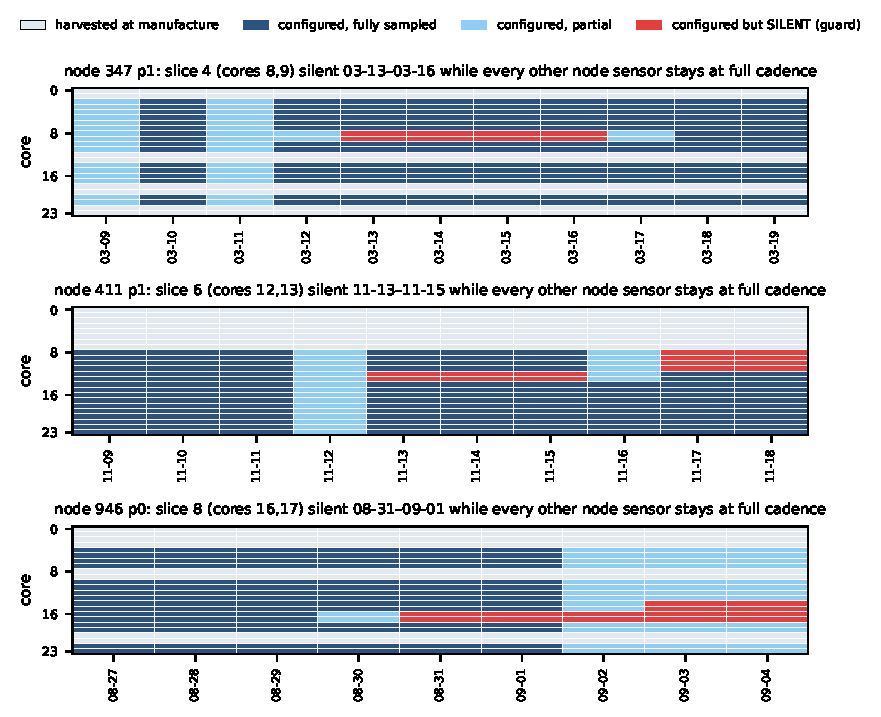
\includegraphics[width=\columnwidth]{f9_guard_episodes.pdf}
\caption{The three core-guard episodes. Grey = harvested at manufacture, blue = configured and
reporting, red = configured but silent. In every case exactly one slice goes silent while all ten
control sensors on the same node stay at full cadence.}\label{fig:guard}\end{figure}

\begin{figure}[t]\centering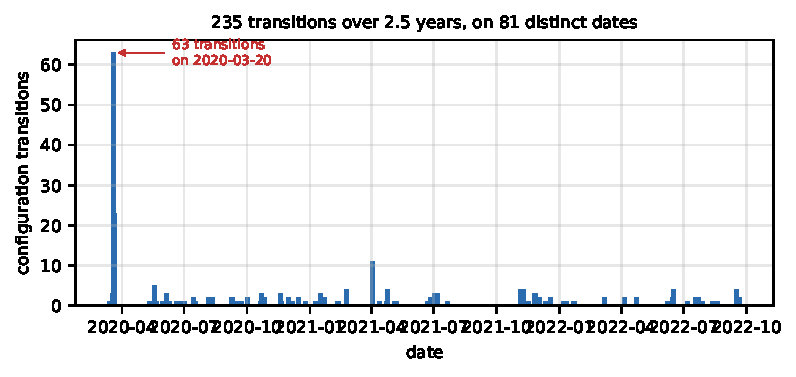
\includegraphics[width=\columnwidth]{f10_transition_dates.pdf}
\caption{Configuration transitions over the full record. 2020-03-20 alone accounts for 63.}
\label{fig:trans}\end{figure}

\begin{figure}[t]\centering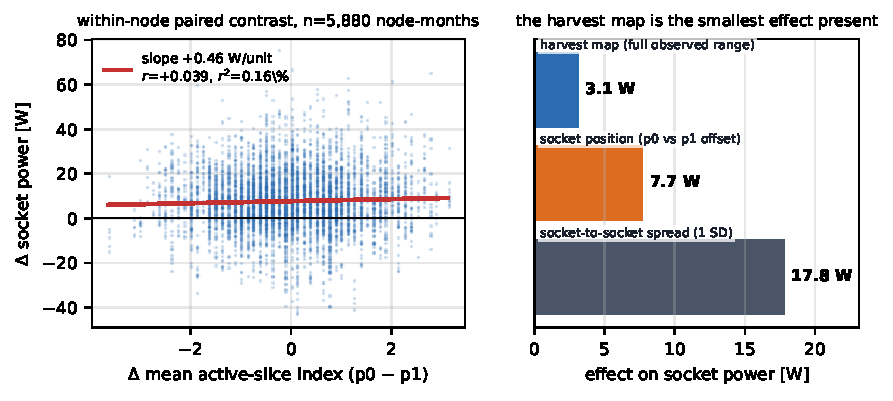
\includegraphics[width=\columnwidth]{f11_operational_impact.pdf}
\caption{Operational impact of the harvest map. Left: within-node paired contrast. Right: the
harvest map's full observed range moves socket power less than half as much as mere socket
position, and a sixth as much as the socket-to-socket spread.}\label{fig:impact}\end{figure}

\section{Threats to validity and open issues}
\label{sec:threats}
Every unresolved item is tracked with an identifier in \texttt{OPEN\_ISSUES.md} in the artefact
repository, which records what is known, what would settle it, and where to look. \textbf{The items
marked \emph{blocking} below must be resolved before this paper is submitted.}

\begin{enumerate}
\item \textbf{Sensor presence $\ne$ core existence.} Mitigated by 99.985\% of 1.67\,M socket-days
reporting exactly 16 cores, agreement with the published 16-core SKU~\cite{ibm_ac922}, the perfect
slice-pair structure, and the control of Sec.~\ref{sec:lifecycle} showing that when core sensors do
vanish, every other sensor on the socket keeps reporting.
\item \textbf{[OI-1, \emph{blocking}] The sensor index may not be the physical die position}
(Sec.~\ref{sec:layout}). The spatial reading of the clustering in Sec.~\ref{sec:cluster} is a
hypothesis, not a result. Needs an annotated die shot or the hostboot sensor-ID mapping.
\item \textbf{[OI-2, \emph{blocking}] A March 2020 BMC firmware update could have remapped sensor
IDs}, mimicking reconfiguration; 86 of the 235 transitions fall in the three days 2020-03-19--21.
Needs CINECA maintenance logs. Does not affect the boot-time-only conclusion.
\item \textbf{[OI-4, \emph{blocking}] Five references are unverified} and a novelty check against
prior telemetry-based binning inference is outstanding.
\item \textbf{[OI-3] Defect-driven versus policy-driven harvesting} cannot be separated from one
machine; both are reported.
\item \textbf{[OI-5] Collection dropout may not be random.} Monthly coverage ranges from 18\% to
99.4\%; if dropout correlates with lot, Sec.~\ref{sec:lot} needs a robustness pass.
\item \textbf{[OI-6, OI-7] both resolved.} The sub-16 socket-days were dominated by an
extraction defect on our side, now gated; the nine that survive are the guard episodes of
Sec.~\ref{sec:lifecycle}. The two nodes appearing to change within a day are same-day reboots.
\item \textbf{[OI-8] The mechanism behind p0/p1 relabelling is unknown}; any per-socket
longitudinal study on this dataset risks silently mixing two dies.
\item \textbf{Common-mode artefact} in the thermal analysis, addressed by same-distance contrasts;
the pooled estimator may be improvable [OI-11].
\item \textbf{[OI-10] Single system}; findings may reflect CINECA procurement rather than POWER9
generally.
\end{enumerate}

\section{Conclusion}
Out-of-band telemetry that supercomputer operators already collect inadvertently publishes a
manufacturing secret: which units a vendor fused off each individual die. Recovering these maps for
1{,}962 POWER9 sockets shows harvesting operates exactly at the slice---the unit sharing an L2/L3
block---with no exceptions in 1.67\,M socket-days; that the maps are per-die rather than per-SKU,
with 443 of 495 possible patterns realised; that harvested slices cluster in sensor-index space;
and that a sharp changepoint at node~440 separates two procurement populations with different
binning statistics. Over 2.5 years the maps are static to within 0.25 percentage points per month,
change only across reboots, and exhibit three field core-guard episodes, each removing exactly one
slice while every other sensor on the socket keeps reporting.

Two boundaries deserve emphasis. We do \emph{not} establish that the sensor index tracks physical
die position, so the clustering result is stated in index space and its spatial reading remains a
hypothesis. And the harvest map turns out to have no measurable operational effect---a negative
result we consider as useful as the positive ones, since it tells operators what they can ignore.
The broader point is that fleet telemetry is a viable instrument for hardware provenance, and that
its unintended disclosures deserve attention from those who publish such datasets.

\section*{Artefact availability}
All analysis code, the derived per-(node, socket, core, day) tables, and the recovered harvest maps
are available at the artefact repository accompanying this paper. Every result is reproducible from
the public M100 ExaData Zenodo releases~\cite{borghesi2023m100}; the derived tables (15\,MB)
suffice for all structural and longitudinal results without re-downloading the 49.9\,TB source.

\bibliographystyle{IEEEtran}
\bibliography{refs}
\end{document}
